\section{Discussion}\label{sec:discussion}

Relative to related works performing trade classification using machine learning, the improvements are strong, as a comparison against \cref{app:literature-ml-tc} reveals.

\textbf{Finding 1: Accuracy of Basic Rules Is Downward-Biased by Coverage}

From \cref{tab:ise-classical} we see, that practically all rule-based approaches leave trades unclassified. This is due to conceptual constraints in the rule itself, but also a result of missing data, which equally affects rules with theoretical full coverage. The latter is important here.

\begin{figure}[!h]
    \centering
    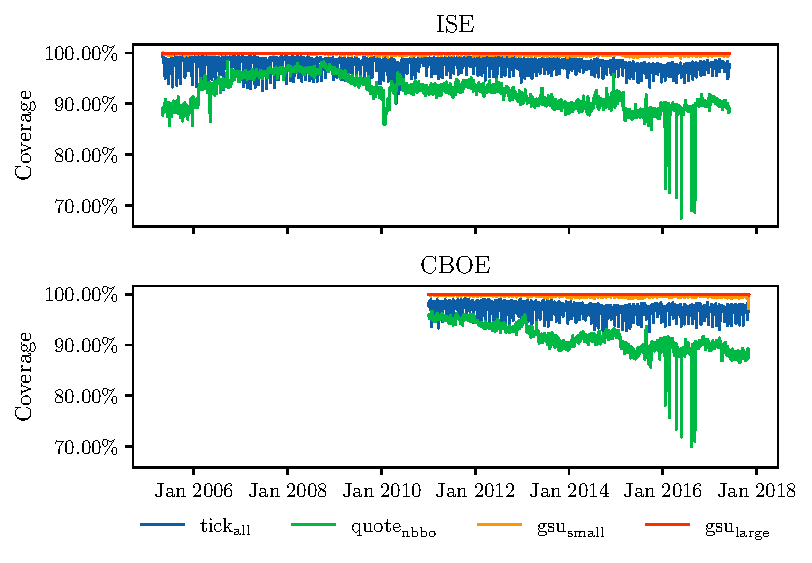
\includegraphics{coverage-over-time.pdf}
    \caption[Coverage of Rule-Based Classifiers Over Time]{Coverage of rule-based classifiers on \gls{ISE} and \gls{CBOE} sample over time. The bar \myline{} indicates the beginning of a new subset based on the train-test split.}
    \label{fig:classical-coverage-over-time}
\end{figure}

\todo{This is not entirely true, as it suggests, that low coverage of quote \gls{NBBO} comes from missing data, but it comes from midspread trades. For the tick rule, I can not distinguish if the trade price was not found, or if it was not different. Rewrite.}

As shown in \cref{fig:classical-coverage-over-time} coverage decreases qualitatively for selected classification rules over time. It is particularly low when the trade initiator is inferred from the \gls{NBBO}. For studies like ours or the of \textcites{grauerOptionTradeClassification2022}[][887]{savickasInferringDirectionOption2003}, which apply minimal filtering, the high degree of unclassified trades for some rules can (downward) bias the results. The recent approaches of \textcite[][18--19]{grauerOptionTradeClassification2022} circumvent the issue, as they leverage multiple data sources and rules through stacking. In an imperfect data regime, we conclude, that stacking can increase coverage and at best performance.

\textbf{Finding 2: Accuracy of Trade Size Rule Is High And Highly Variant}

\todo{Missclassification bias, as some trades are perfectly classified, why others are not improved?}

Much of the performance gains between $\operatorname{gsu}_{\mathrm{large}}$ over $\operatorname{gsu}_{\mathrm{small}}$ in \cref{fig:classical-accuracies-over-time} can be attributed to the trade size rule. We extend the analysis of \textcite[][19]{grauerOptionTradeClassification2022} and isolate the performance of the trade size rule and visualise the average accuracy over time in \cref{fig:accuracies-over-time-tsize}.

\begin{figure}[!h]
    \centering
    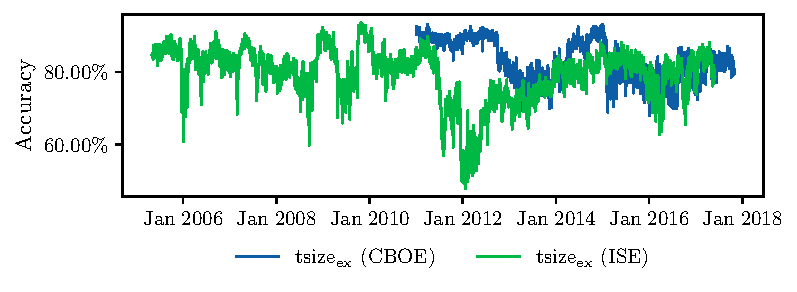
\includegraphics{accuracies-over-time-tsize.pdf}
    \caption[Accuracy and Coverage of Trade Size Rule Over Time]{Accuracy and Coverage of trade size rule on \gls{ISE} and \gls{CBOE} sample over time. The bar \myline{} indicates the beginning of a new subset based on the train-test split.}
    \label{fig:accuracies-over-time-tsize}
\end{figure}

For the subset of trades it is applicable to, the rule is outperforming all other rule-based classifiers by a large margin. At the same time, it also has the highest variance in accuracy over time with sharp drops in accuracy to \SI{47.991543}{\percent}. Thus, it remains unclear, under which circumstances the rule works reliably.

\textbf{Finding 4: Classifier Performance on \gls{CBOE}}

\todo{Formulate finding.}

\textbf{Finding 5: Link Between Unlabelled Trades And Generalisation Performance}

\todo{Formulate finding.}


\newpage
\section{Conclusion}\label{sec:conclusion}

\todo{The predictability results survive an extensive list of robustness checks. Make clear we compare deep learning vs tree-based methods. None is superior.}

The goal of this study is to examine the performance of machine learning-based trade classification in the option market. In particular, we propose to model trade classification with Transformers and gradient boosting. Both approaches are supervised and leverage labelled trades. For settings, where labelled trades are scarce, we extend Transformers with a pre-training objective to train on unlabelled trades as well as generate pseudo-labels for gradient boosting through a self-training procedure.

Our models establish a new state-of-the-art for trade classification on the \gls{ISE} and \gls{CBOE} dataset. For \gls{ISE} trades, Transformers achieve an accuracy of \SI{63.78}{\percent} when trained on trade and quoted prices as well as \SI{72.58}{\percent} when trained on additional quoted sizes, improving over current best of \textcite[][27]{grauerOptionTradeClassification2022} by \SI{3.73}{\percent} and \SI{4.97}{\percent}. Similarly, \glspl{GBRT} reach accuracies between \SI{63.67}{\percent} and \SI{73.24}{\percent}. We observe performance improvements up to \SI{6.51}{\percent} for \glspl{GBRT} and \SI{6.31}{\percent} for Transformers when models have access to option characteristics. Relative to the ubiquitous tick test, quote rule, and LR algorithm, improvements are \SI{23.88}{\percent}, \SI{17.11}{\percent}, and \SI{17.02}{\percent}. Outperformance is particularly strong for \gls{OTM} options, options with a long maturity, as well as options traded at the quotes. Both architectures generalise well on \gls{CBOE} data, with even stronger improvements between \SI{4.92}{\percent} and \SI{7.58}{\percent} over the benchmark depending on the model and feature set. 

In the semi-supervised setting, Transformers on \gls{ISE} dataset profit from pre-training on unlabelled trades with accuracies up to \SI{74.55}{\percent}, but the performance gains slightly diminish on the \gls{CBOE} test set. Vice versa, we observe no benefits from semi-supervised training of \glspl{GBRT}.
% Consistent with \textcites[][27]{grauerOptionTradeClassification2022}[][901]{savickasInferringDirectionOption2003} we find evidence that the performance of common trade classification rules deteriorates in the option market. In particular, tick-based methods marginally outperform a random guess.

Unlike previous studies, we can trace back the performance of our approaches as well as of trade classification rules to individual features and feature groups using the importance measure \gls{SAGE}. We find that both paradigms attain the largest performance improvements from classifying trades based on quoted sizes and prices, but machine learning-based classifiers attain higher performance gains and effectively exploit the data. The change in the trade price, decisive criteria to the (reverse) tick test, plays no role in option trade classification. We identify the relative illiquidity of options to affect the information content of the surrounding trade prices. Our classifiers profit from the inclusion of option-specific features, like moneyness and time-to-maturity, currently unexploited in classical trade classification.

By probing and visualising the attention mechanism of the Transformer, we can establish a connection to rule-based classification. Graphically, our results show, that attention heads encode knowledge about rule-based classification. Whilst attention heads in earlier layers of the network broadly attend to all features or their embeddings, later they focus on specific features jointly used in rule-based classification akin to the \gls{LR} algorithm, depth rule or others. Furthermore, embeddings encode domain knowledge. Our results demonstrate exemplary for traded underlying, that the Transformer learns to group similar underlyings in embedding space.

Our classifiers deliver accurate predictions and improved robustness, which effectively reduces noise and bias in option research dependent on reliable trade initiator estimates. When applied to measuring trading cost through effective spreads, the models dominate all rule-based approaches by approximating the true effective spread of options best. Exemplary, the Transformer pre-trained on unlabelled trades estimates a mean spread of  \SI[round-mode=places, round-precision=3]{0.013118}[\$]{} versus \SI[round-mode=places, round-precision=3]{0.004926}[\$]{} actual spread at the \gls{ISE}.

In conclusion, our study showcases the efficacy of machine learning as a viable alternative to existing trade signing algorithms for classifying option trades, if partially-labelled or labelled trades are available for training. % While we tested our models on option trades, we expect the results to transfer to other modalities including equity trades. 

\newpage
\section{Outlook}\label{sec:outlook}

In future work, we plan to revisit training Transformers on a larger corpus of unlabelled trades through pre-training objectives and study the effects from \emph{exchange-specific} finetuning. While our current results show that pre-training positively drives classification performance, for comparability it is only performed on a small subset of trades and models have not fully converged. Thus, we expect to see benefits from additional data and compute, following the scaling laws of \textcite[][7]{hoffmannTrainingComputeOptimalLarge2022}. The application confers advantages when finetuning is constrained due to the limited availability of the true trade initiator.

Indicatively, our results show that specific attention heads in the Transformer specialise in patterns akin to classical trade classification rules. We want to explore this aspect further and potentially reverse engineer classification rules from attention heads that are yet unknown. This way, we can transfer the superior classification accuracy of the Transformer to regimes where labels are unavailable or computational costs of training are not affordable.